\chapter{Related Work}

\section{Tokenization}
Tokens are the fundamental units of data processing in natural language processing (NLP). A token is the smallest meaningful unit of text, which can be a word, subword, or even a single character or punctuation mark. Tokenization is typically performed at one of three levels: single characters (character-based tokenization), subwords (subword-based tokenization), or whole words (word-based tokenization).

In most modern NLP models, subword tokenization is predominantly used. This technique breaks words into smaller units, such as prefixes and suffixes. Unlike word-based tokenizers, which generate a very large vocabulary and suffer from a loss of meaning across very similar words as well as a large quantity of out-of-vocabulary tokens, or character-based tokenization, where each token has minimal meaning in context and the overall number of tokens on a tokinzed text is enormous, subword-based tokenization seeks to find a middle ground. The idea is to decompose rare words into meaningful subwords while maintaining few to single tokens for every meaningful or frequently used word.

Subword tokenizers are employed in almost every widely-used large language model (LLM) such as GPT-2, Llama 3, and in large pre-trained language models like BERT.

% https://huggingface.co/docs/transformers/en/tokenizer_summary


\section{The Transformer}
The Transformer architecture, introduced in June 2017, marked a significant advancement in natural language processing (NLP), initially focusing on sequence-to-sequence NLP problems like machine translation tasks. However, its capabilities quickly revealed a broader potential, particularly in developing large language models (LLMs). These models are trained on vast amounts of raw text using self-supervised learning, a method where the training objective is derived automatically from the input data. After that the model developed a statistically understanding of the language but still needs to be improved by e.g. masked language-modeling or causal language modeling. The Tranformer consists of a encoder and a decoder.
% https://arxiv.org/abs/1706.03762



\begin{figure}[h]
    
    \centering
    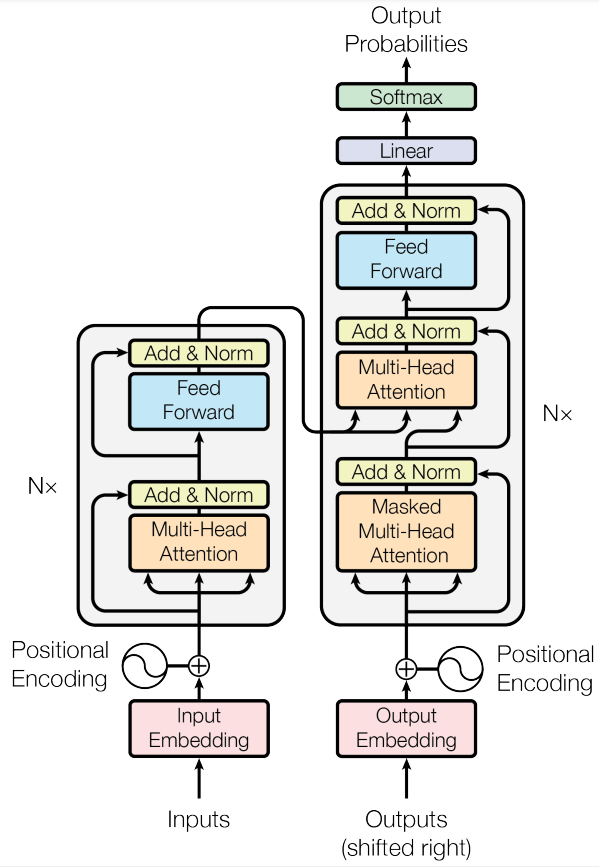
\includegraphics[width=6cm]{ressources/images/Transformer.png}
    \caption{transformer architecture from the original paper}
    \end{figure}
\subsection{Encoder}
The encoder takes an input sequence, and breaks it down into individual tokens (words or sub-words).
For each token an embedding vector is computed, which is a numerical representation of that token, capturing its semantic meaning.

A key component of the encoder is the self-attention mechanism. Self-attention enables the model to consider the entire sequence when encoding each token, allowing it to weigh the relevance of other tokens in the input sequence dynamically. For each token, the self-attention mechanism computes attention scores that determine the influence of all other tokens in the sequence. So the generated embedded vector for each token does not only represent the token alone but also its left and right contextual influence.


The encoder consists of multiple identical layers, or encoder blocks. Each encoder block contains two main sub-layers:

\begin{itemize}
    \item \textbf{Multi-Head Self-Attention Layer}: This sub-layer allows the model to attend to different parts of the sequence from multiple perspectives or "heads." Each head performs self-attention independently, and their outputs are concatenated and linearly transformed to provide a richer representation.

    \item \textbf{Feed-Forward Layer}: After the self-attention sub-layer, each token's representation is passed through a feed-forward neural network. This layer is a simple fully connected feed-forward network applied to each position (word) in the sequence independently and identically. It consists of two linear transformations with a ReLU activation in between, allowing the model to apply non-linear transformations and further refine the encoded representation.
\end{itemize}

Both sub-layers in the encoder block are followed by residual connections and layer normalization, which help in stabilizing the training and improving convergence.

\subsection{Decoder}
The decoder works quiet similar to the encoder and can be also be used for same tasks but with respect to loss of performance. It also uses multiple decoder blocks, similar to the encoder but has two additional sub-layers per block as compared to the encoder block. In the transformer's architecture the decoder's role is to generate the output sequence based on the encoded representation from the encoder (cross-attention). This is done auto-regressively, which means that the generated computed feature-vector, which holds information about the input sequence will be tranformed by the language modelling head mapping into the next probable following word, which then will be added to the input text and then get feeded back into the decoder. The most important difference to the encoder is the masked multi-head self-attention.

\begin{itemize}
    \item \textbf{Masked Multi-Head Self-Attention Layer}:
          Since the decoder cannot predict future words based on information not yet generated, it only attends uni-directional to the previously generated tokens in the output sequence. Therfor only the left context (for "LTR" text) is used and the right context is masked.
\end{itemize}





\section{BERT}
BERT (Bidirectional Encoder Representations from Transformers) is a  pre-trained language representation model introduced by Devlin et al. in 2019 (ref). Its based on the Transformer architecture from\dots but instead of using in contrast to using both, an encoder and a decoder as in the original transformer, BERT only utilizes the encoder component. Consequently, unlike other large language models (LLMs), BERT cannot predict new tokens and thus is not suitable for text generation. Instead, it still achieves state-of-the-art results in tasks such as text classification, sentiment analysis, and named entity recognition. The attention scores are computed using queries, keys, and values derived from the input embeddings.

\subsection{Embeddings}
The three matrices in BERT—token embeddings, segment embeddings, and positional embeddings are generated as part of the model's training process.

For each unique Token ID (i.e. for each of the 30,522 words and subwords in the BERT Tokenizer’s vocabulary), the BERT model contains an embedding that is trained to represent that specific token. The Embedding Layer within the model is responsible for mapping tokens to their corresponding embeddings.

Before a string of text is passed to the BERT model, the BERT Tokenizer is used to convert the input from a string into a list of integer Token IDs, where each ID directly maps to a word or part of a word in the original string. In addition to the Token Embeddings described so far, BERT also relies on Position Embeddings. While Token Embeddings are used to represent each possible word or subword that can be provided to the model, Position Embeddings represent the position of each token in the input sequence.

The final type of embedding used by BERT is the Token Type Embedding, also called the Segment Embedding in the original BERT Paper. One of the tasks that BERT was originally trained to solve was Next Sentence Prediction. That is, given two sentences A and B, BERT was trained to determine whether B logically follows A.\\

BERT introduces two pre-training objectives, the masked language model objective (MLM), and the next sentence prediction objective (NSP).


\begin{itemize}
    \item \textbf{Masked Language Modeling (MLM)}:
          15\% of the words in a sentence are randomly masked, and the model is trained to predict these masked words based on the context provided by the other words in the sentence. This enables BERT to learn bidirectional representations.

    \item \textbf{Next Sentence Prediction (NSP)}:
          To understand relationships between sentences, BERT is trained on pairs of sentences. Given two sentences, the model predicts whether the second sentence is the actual next sentence in the original text or a randomly chosen one. This task helps BERT capture the coherence and context between sentences.
\end{itemize}


\subsection{Fine-Tuning}
After pre-training on large text corpora, BERT can be fine-tuned on specific downstream tasks with relatively small amounts of data. Fine-tuning involves adjusting the pre-trained model weights slightly to better fit the target task. This approach leverages the robust pre-trained language representations and adapts them to the specific requirements of the task at hand.




\subsection{BERTScore}
BERTScore is an evaluation metric that utilizes the BERT model to compare texts more semantically than traditional metrics like BLEU. It leverages the contextualized embeddings provided by a pre-trained BERT model to assess the similarity between candidate and reference texts.\\

The process begins by inputting both candidate and reference texts into the BERT model, which generates contextualized embeddings for each token in both texts. For each token, the similarity between its embedding and every token embedding in the comparison text is calculated using cosine similarity
\begin{equation}
    \cos(\theta) = \frac{\mathbf{A} \cdot \mathbf{B}}{\|\mathbf{A}\| \|\mathbf{B}\|} = \frac{\sum_{i=1}^{n} \mathbf{A}_{i} \mathbf{B}_{i} }{\sqrt{\sum_{i=1}^{n} \mathbf{A}_{i}} \cdot \sqrt{\sum_{i=1}^{n} \mathbf{B}_{i}} }
\end{equation}
This results in a similarity matrix where each entry represents the cosine similarity between the embeddings of a pair of tokens (one from the candidate sentence and one from the reference sentence).\\


The metric is computed symmetrically as follows:\\

For each token embedding in the candidate sentence, find the maximum similarity score with any token embedding in the reference sentence, and average these scores across all tokens in the candidate sentence to obtain precision.\\

Similarly, for each token embedding in the reference sentence, find the maximum similarity score with any token embedding in the candidate sentence, and average these scores across all tokens in the reference sentence to obtain recall.

\[P_{BERT} = \frac{1}{|\hat{x}|} \sum_{\hat{x}_j\in \hat{x}} \max_{x_i \in x} x_i^T \hat{x_j} \]
\[R_{BERT} = \frac{1}{|x|} \sum_{x_i \in x} \max_{\hat{x}_j\in \hat{x}} x_i^T \hat{x_j} \]



Finally the $F_1$-score (an $F$-measure)
is computed as the harmonic mean of precision and recall and is providing a balanced measure that considers both the model's ability to capture relevant information and its accuracy in predicting new text equally.

\[F_{BERT} = 2\frac{P_{BERT}R_{BERT}}{P_{BERT} + R_{BERT}} \]

\section{BLEU-Score}

BLEU-Score is a different metric I use in my thesis for comparing texts. BLEU is not evaluating and comparing the semantic of the reference and candidate text but instead comparing similarity of vocabulary between them.

Let $\left\{y^{1}, y^{2}, ..., y^{N}\right\}$ be the words of the reference text and $\left\{\hat{y}^{1}, \hat{y}^{2}, ..., \hat{y}^{N}\right\}$


The first step is to create n-grams $\text{G}_n(y)$ for both texts. An n-gram is just a set of consecutive words of length n in a text.

\[
    \text{G}_n(y) = \left\{y_1, y_2, ..., y_k\right\}
\]

Next we define the function $\text{C}(s,y)$ that counts the appearances of s as a substring in y.
Now we can count n-grams of the candidate that appear in the reference text. We can compute the clipped precision by taking the minimum of the appearances of the n-gram in $y$ and $\hat{y}$ and then dividing by the amount of all occurences of n-grams in $\hat{y}$. Therefor candidates that have the same n-gram repeating over and over again don't get a higher precision score if the same n-gram does not appear in the reference text the same amount.

\[
    \text{p}_n(\hat{y} , y) = \frac{\sum_{s \in G_n(\hat{y})} \min(\text{C}(s,\hat{y}), \text{C}(s,y))}{\sum_{s \in G_n(\hat{y})} \text{C}(s,\hat{y})}
\]


Right now short candidate texts are more likely to get a good score although the reference text is much longer. Therefor we add a brevity penalty in order to give higher scores to texts that are closer or even longer to the reference texts real size.
\[
    \text{BP}(c, r) = \left\{\begin{array}{lr}
        1,               & \text{if } c > r    \\
        \ e^{(1 - r/c)}, & \text{if } c \leq r \\
    \end{array}\right\}
\]

Finally for BLEU-Score we combine the brevity penalty with the clipped precision of n-grams. We additionally add a distribution vector to weigh each $ \text{p}_n$ by $w_n$ in order to have the opportunity to give n-grams with different $n$ also a different impact on the overall result. Although in the end most BLEU-Scores just use a uniform distribution with $N = 4$ so that $w_n$ always stays $\frac{1}{4}$

\[\text{BLEU} = \text{BP}(c, r) \cdot \exp\left(\sum_{n=1}^{N}  \text{w}_n \cdot \ln(p_n)\right)\]

